
Este capítulo apresenta em detalhes toda a concepção e implementação técnica do projeto MatchPredict-AI. As seções a seguir descrevem as fontes de dados e o processo de curadoria, o complexo pipeline de engenharia de features, a arquitetura de rede neural em grafos utilizada e, por fim, o desenho experimental que fundamenta a análise de resultados.

% --- Inclusão das Subseções ---
% Assumindo que os arquivos de conteúdo estão na mesma pasta 'tex/'
% Se você os colocou em uma subpasta como 'tex/desenvolvimento/', ajuste o caminho.
% Exemplo: % tex/Desenvolvimento/dev_01_fontes_dados.tex
\section{Fontes de Dados e Construção do Dataset}
\label{sec:dev_fontes_dados}

\textbf{Estratégia de Coleta e Fusão:} \\
A construção de um sistema de recomendação robusto e eficaz, como o MatchPredict-AI, depende fundamentalmente da qualidade e da diversidade dos dados utilizados para treinamento e avaliação. A premissa central deste trabalho é que a afinidade em relacionamentos é um fenômeno multimodal, influenciado por uma complexa interação de fatores textuais, demográficos e visuais. Para capturar essa complexidade, a estratégia adotada foi a fusão de dois conjuntos de dados públicos distintos, cada um especializado em uma modalidade de informação, visando criar um dataset final de 2000 perfis que fosse completo e rico em características.

\subsection{Dataset de Conteúdo Textual e Demográfico: OkCupid}
\textbf{Descrição:} \\
A base para os dados comportamentais e demográficos foi extraída de uma versão pública do dataset do **OkCupid**. Esta fonte de dados é amplamente reconhecida na comunidade de pesquisa por sua riqueza em informações auto-descritivas fornecidas pelos usuários no formato de ensaios textuais. Para este trabalho, foi utilizado especificamente o campo `essay0`, que corresponde à biografia principal onde os usuários se descrevem livremente. Este texto aberto é um recurso valioso para a aplicação de técnicas de Processamento de Linguagem Natural (PLN) para inferir interesses, estilo de comunicação e até traços de personalidade.

\textbf{Contextualização e Uso:} \\
Além do conteúdo textual, o dataset OkCupid fornece dados demográficos estruturados, como idade e sexo, que foram diretamente incorporados como features no nosso modelo. A natureza inerentemente heterogênea do dataset OkCupid -- combinando texto não estruturado com atributos categóricos e numéricos -- o torna uma fonte ideal para a extração de um conjunto abrangente de features descritivas dos perfis, fundamentais para a modelagem da compatibilidade.

\subsection{Dataset de Conteúdo Visual: SCUT-FBP5500}
\textbf{Descrição:} \\
Para o componente visual, que desempenha um papel inegável na formação de interesse inicial em plataformas de relacionamento, foi incorporado o dataset **SCUT-FBP5500 (Facial Beauty Prediction)** \textcolor{blue}{[\cite{wang2018scut}]}. Trata-se de um dataset de benchmark público e amplamente utilizado na pesquisa de predição de beleza facial. Ele é composto por 5500 imagens faciais frontais, com diversidade de gênero (masculino/feminino) e etnia (asiáticos e caucasianos), cada uma acompanhada por um escore de beleza atribuído por múltiplos avaliadores.

\textbf{Contextualização e Uso:} \\
A utilização deste dataset especializado como fonte para as imagens dos perfis permitiu a associação de imagens de alta qualidade e com iluminação controlada aos perfis textuais do OkCupid. A premissa é que, ao extrair features visuais dessas imagens através de modelos de visão computacional, seria possível capturar elementos relacionados à atratividade física, um componente que, embora subjetivo, é de grande importância no contexto do projeto.

\subsection{Processo de Curadoria e Fusão do Dataset Final}
\textbf{Explicação Detalhada:} \\
A criação do conjunto de dados final de 2000 perfis envolveu um processo criterioso de mapeamento, seleção e combinação. O objetivo foi assegurar que cada uma das 2000 instâncias finais contivesse um conjunto completo e alinhado de informações multimodais. O processo, implementado no script `src/models/features.py`, consistiu em parear os perfis do OkCupid com as imagens do SCUT-FBP5500, utilizando um sistema de indexação para encontrar correspondências.

O critério de inclusão para um perfil no dataset final era rigoroso: o perfil deveria possuir simultaneamente (1) um ensaio textual (`essay0`) não nulo e (2) uma imagem correspondente válida e localizada no sistema de arquivos. Perfis que não atendiam a ambos os requisitos foram descartados. Este processo de seleção e combinação buscou garantir não apenas a quantidade, mas também a integridade e a diversidade necessárias para treinar um modelo de recomendação capaz de aprender padrões complexos, evitando vieses que poderiam surgir de amostras de dados incompletas ou homogêneas.

% tex/Desenvolvimento/dev_01_fontes_dados.tex
\section{Fontes de Dados e Construção do Dataset}
\label{sec:dev_fontes_dados}

\textbf{Estratégia de Coleta e Fusão:} \\
A construção de um sistema de recomendação robusto e eficaz, como o MatchPredict-AI, depende fundamentalmente da qualidade e da diversidade dos dados utilizados para treinamento e avaliação. A premissa central deste trabalho é que a afinidade em relacionamentos é um fenômeno multimodal, influenciado por uma complexa interação de fatores textuais, demográficos e visuais. Para capturar essa complexidade, a estratégia adotada foi a fusão de dois conjuntos de dados públicos distintos, cada um especializado em uma modalidade de informação, visando criar um dataset final de 2000 perfis que fosse completo e rico em características.

\subsection{Dataset de Conteúdo Textual e Demográfico: OkCupid}
\textbf{Descrição:} \\
A base para os dados comportamentais e demográficos foi extraída de uma versão pública do dataset do **OkCupid**. Esta fonte de dados é amplamente reconhecida na comunidade de pesquisa por sua riqueza em informações auto-descritivas fornecidas pelos usuários no formato de ensaios textuais. Para este trabalho, foi utilizado especificamente o campo `essay0`, que corresponde à biografia principal onde os usuários se descrevem livremente. Este texto aberto é um recurso valioso para a aplicação de técnicas de Processamento de Linguagem Natural (PLN) para inferir interesses, estilo de comunicação e até traços de personalidade.

\textbf{Contextualização e Uso:} \\
Além do conteúdo textual, o dataset OkCupid fornece dados demográficos estruturados, como idade e sexo, que foram diretamente incorporados como features no nosso modelo. A natureza inerentemente heterogênea do dataset OkCupid -- combinando texto não estruturado com atributos categóricos e numéricos -- o torna uma fonte ideal para a extração de um conjunto abrangente de features descritivas dos perfis, fundamentais para a modelagem da compatibilidade.

\subsection{Dataset de Conteúdo Visual: SCUT-FBP5500}
\textbf{Descrição:} \\
Para o componente visual, que desempenha um papel inegável na formação de interesse inicial em plataformas de relacionamento, foi incorporado o dataset **SCUT-FBP5500 (Facial Beauty Prediction)** \textcolor{blue}{[\cite{wang2018scut}]}. Trata-se de um dataset de benchmark público e amplamente utilizado na pesquisa de predição de beleza facial. Ele é composto por 5500 imagens faciais frontais, com diversidade de gênero (masculino/feminino) e etnia (asiáticos e caucasianos), cada uma acompanhada por um escore de beleza atribuído por múltiplos avaliadores.

\textbf{Contextualização e Uso:} \\
A utilização deste dataset especializado como fonte para as imagens dos perfis permitiu a associação de imagens de alta qualidade e com iluminação controlada aos perfis textuais do OkCupid. A premissa é que, ao extrair features visuais dessas imagens através de modelos de visão computacional, seria possível capturar elementos relacionados à atratividade física, um componente que, embora subjetivo, é de grande importância no contexto do projeto.

\subsection{Processo de Curadoria e Fusão do Dataset Final}
\textbf{Explicação Detalhada:} \\
A criação do conjunto de dados final de 2000 perfis envolveu um processo criterioso de mapeamento, seleção e combinação. O objetivo foi assegurar que cada uma das 2000 instâncias finais contivesse um conjunto completo e alinhado de informações multimodais. O processo, implementado no script `src/models/features.py`, consistiu em parear os perfis do OkCupid com as imagens do SCUT-FBP5500, utilizando um sistema de indexação para encontrar correspondências.

O critério de inclusão para um perfil no dataset final era rigoroso: o perfil deveria possuir simultaneamente (1) um ensaio textual (`essay0`) não nulo e (2) uma imagem correspondente válida e localizada no sistema de arquivos. Perfis que não atendiam a ambos os requisitos foram descartados. Este processo de seleção e combinação buscou garantir não apenas a quantidade, mas também a integridade e a diversidade necessárias para treinar um modelo de recomendação capaz de aprender padrões complexos, evitando vieses que poderiam surgir de amostras de dados incompletas ou homogêneas.
% tex/desenvolvimento/dev_02_pipeline_features.tex
\section{Pipeline de Engenharia de Features}
\label{sec:dev_pipeline_features}

\sloppy

\textbf{Definição:} \\
A transformação dos dados brutos multimodais em um formato numérico, denso e semanticamente rico é uma etapa fundamental e crítica em qualquer projeto de aprendizado de máquina. Para o MatchPredict-AI, o objetivo deste pipeline foi a criação de um vetor de características de alta dimensionalidade, especificamente com \textbf{2503 dimensões}, para cada um dos 2000 perfis. Este vetor robusto visa encapsular as múltiplas facetas de um perfil de usuário, desde sua aparência e auto-descrição textual até sua posição no ecossistema social de perfis. O processo completo está implementado em um conjunto de scripts modulares, principalmente \texttt{src/models/features.py}, \texttt{src/models/social\_graph.py} e \texttt{src/models/combine\_features.py}. A Figura~\ref{fig:pipeline_dados_tcc2} ilustra o fluxo geral deste pipeline.

\begin{figure}[h!]
    \centering
    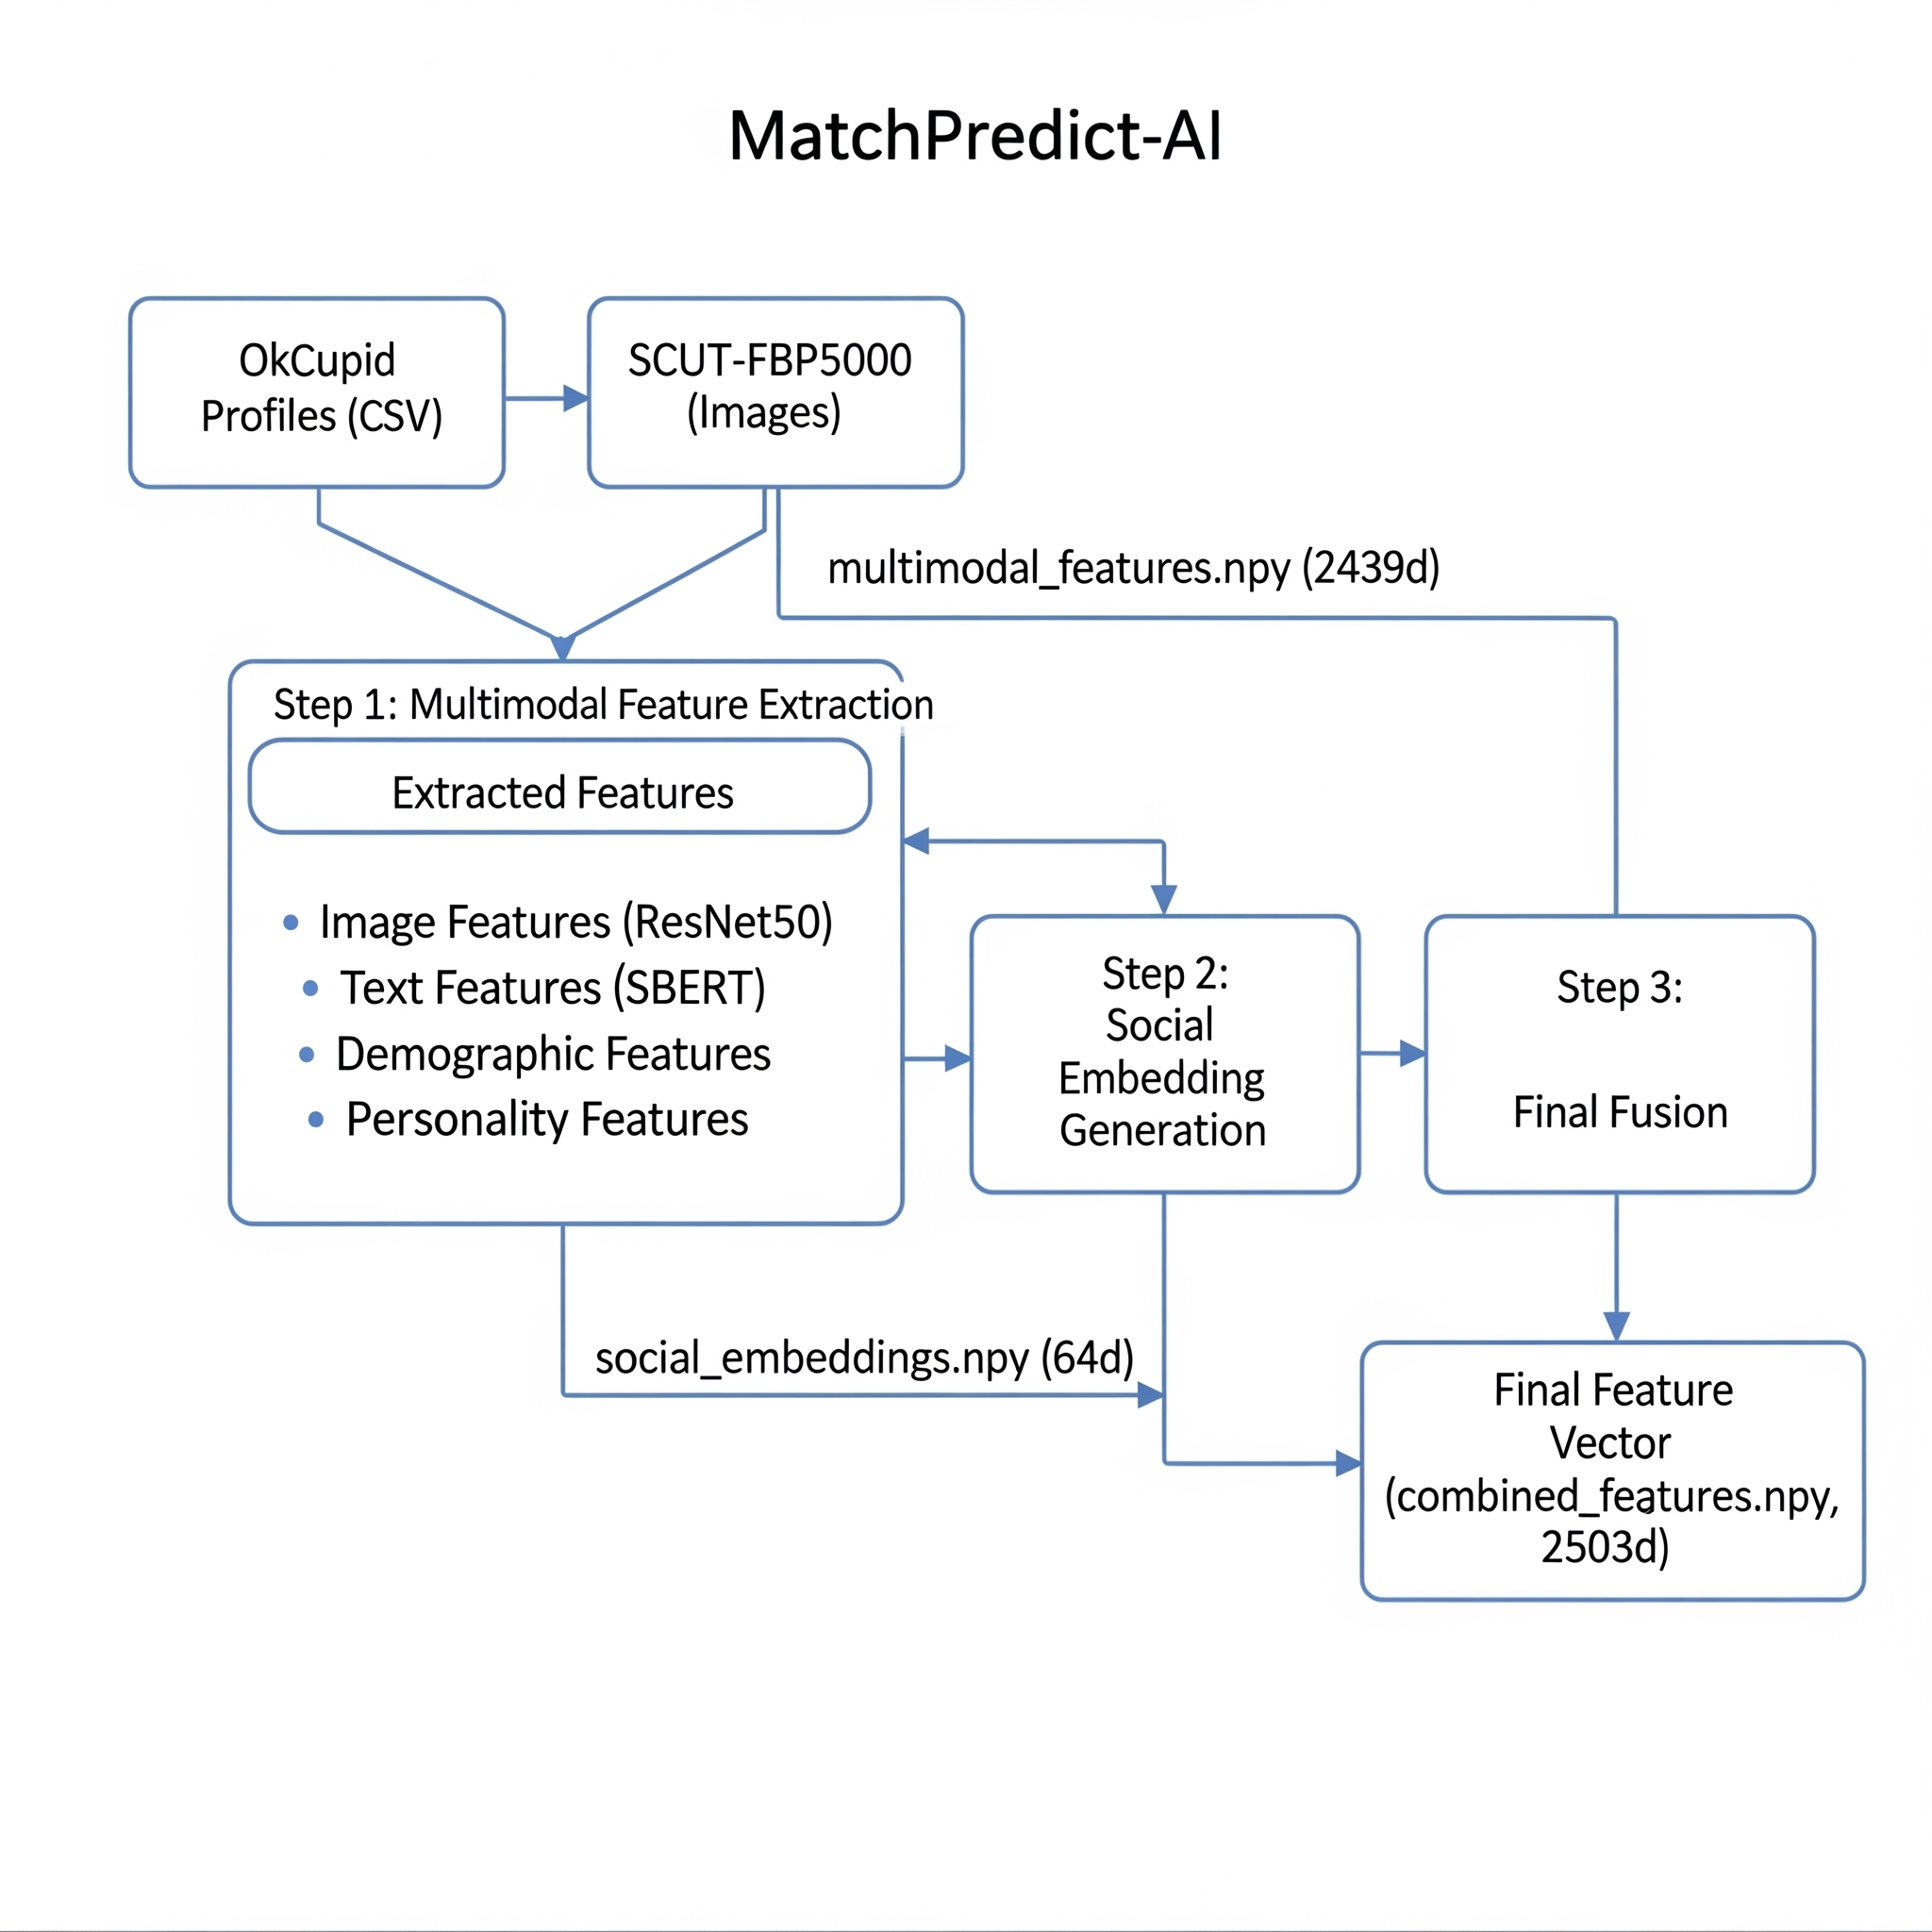
\includegraphics[width=\textwidth]{imagens/diagrama_pipeline.png}
    \caption{Diagrama do pipeline de engenharia de features, ilustrando o fluxo desde os dados brutos até a composição do vetor final de 2503 dimensões.}
    \label{fig:pipeline_dados_tcc2}
\end{figure}

\subsection{Extração de Features Multimodais (2439 dimensões)}
\textbf{Implementação (\texttt{src/models/features.py}):} \\
A primeira fase do pipeline é responsável por processar as diferentes modalidades de dados (imagem, texto, etc.) e convertê-las em representações vetoriais.

\begin{itemize}
    \item \textbf{Features de Imagem (2048 dimensões):} As características visuais de cada perfil foram extraídas utilizando uma Rede Neural Convolucional (CNN) \textbf{ResNet50}, pré-treinada no vasto dataset ImageNet. A escolha da ResNet50 se deve ao seu reconhecido balanço entre profundidade arquitetural e capacidade de extrair features hierárquicas complexas. Em vez de usar a saída final do modelo, foi utilizado o vetor de ativação da penúltima camada (a camada de \textit{average pooling}), que resulta em um embedding de 2048 dimensões. Esta técnica de \textit{transfer learning} permite capturar características visuais abstratas e de alto nível (como formas, texturas e composições) que são mais úteis para tarefas de similaridade do que as classes finais da ImageNet.

    \item \textbf{Features de Texto (384 dimensões):} Para converter as biografias textuais (\texttt{essay0}) em vetores numéricos, foi empregado o modelo \textbf{Sentence-BERT}, especificamente a variante \texttt{all-MiniLM-L6-v2}. Esta arquitetura baseada em Transformers é projetada para gerar embeddings de sentenças que capturam o significado semântico do texto de forma contextualizada. O resultado é um vetor de 384 dimensões que representa a essência da auto-descrição do usuário, uma melhoria significativa sobre métodos mais antigos como Bag-of-Words, que ignoram o contexto e a semântica.

    \item \textbf{Features Demográficas (2 dimensões):} Dois dados demográficos foram incluídos: a idade, que foi normalizada para o intervalo $[0,1]$ para manter a consistência de escala com as outras features; e o sexo, que foi codificado numericamente (por exemplo, $0$ para masculino, $1$ para feminino).

    \item \textbf{Features de Personalidade (5 dimensões):} Para inferir traços de personalidade, foi implementado um método simples e eficaz baseado em léxico no script \texttt{src/models/personality.py}. Um dicionário de palavras-chave foi criado, associando termos a cada um dos cinco grandes traços de personalidade (``Big Five'': Abertura, Conscienciosidade, Extroversão, Amabilidade e Neuroticismo). O texto da biografia de cada usuário é então escaneado, e a frequência normalizada de palavras de cada categoria gera um vetor de 5 dimensões. Este vetor serve como uma aproximação do perfil psicológico do usuário, baseada em como ele se descreve.
\end{itemize}

Ao final desta fase, o vetor multimodal de 2439 dimensões é salvo no arquivo \texttt{multimodal\_features.npy}.

\subsection{Geração de Embeddings Sociais (64 dimensões)}
\textbf{Adaptação Metodológica:} \\
A proposta original do TCC1 considerava o uso de APIs de redes sociais (como a do Instagram) para construir um grafo social explícito, onde as arestas representariam amizades ou seguidores. Contudo, na prática, essa abordagem apresenta desafios significativos, como restrições de acesso a APIs, questões de privacidade do usuário e a dificuldade de mapear identidades entre diferentes plataformas. Para superar essa barreira, foi adotada uma solução alternativa, implementada em \texttt{src/models/social\_graph.py}: a criação de um \textbf{grafo social implícito}, baseado na similaridade entre os próprios perfis do nosso dataset. Esta abordagem é metodologicamente robusta, autocontida e define ``conexões sociais'' como uma alta afinidade de características entre os perfis.

\textbf{Implementação (\texttt{src/models/social\_graph.py}):}
\begin{enumerate}
    \item \textbf{Construção do Grafo de Similaridade:} Primeiramente, um grafo não-direcionado foi construído, onde os 2000 perfis do nosso dataset são os nós. Para criar as arestas, foi utilizado o algoritmo \textbf{K-Nearest Neighbors (KNN)}. Para cada perfil (nó), foram identificados os seus $k=10$ vizinhos mais próximos no espaço de features de 2439 dimensões. A métrica de proximidade utilizada foi a \textbf{similaridade de cosseno}, que é eficaz para medir a semelhança entre vetores de alta dimensionalidade. O resultado é um grafo onde as arestas conectam perfis que são muito parecidos em termos de imagem, texto, demografia e personalidade.

    \item \textbf{Aprendizado de Representação com Node2Vec:} Com o grafo de similaridade construído, o passo seguinte foi aprender uma representação vetorial (embedding) para cada nó que capturasse a topologia do grafo. Para isso, foi utilizado o algoritmo \textbf{Node2Vec}. Este algoritmo realiza ``caminhadas aleatórias'' (random walks) no grafo para gerar sequências de nós. Em seguida, ele aplica um modelo da família Word2Vec (especificamente, Skip-Gram) sobre essas sequências para aprender um embedding de baixa dimensionalidade – neste caso, 64 dimensões – para cada nó. O vetor resultante para um perfil não descreve mais suas características intrínsecas, mas sim sua \textbf{posição e papel estrutural dentro da rede de perfis similares}.
\end{enumerate}

Este processo, que culmina na criação do arquivo \texttt{social\_embeddings.npy}, é fundamental para o componente \texttt{ItemModel} da arquitetura GraphRec.

\subsection{Fusão Final do Vetor de Features}
\textbf{Implementação (\texttt{src/models/combine\_features.py}):} \\
A etapa final do pipeline é a simples, porém crucial, concatenação dos vetores de features gerados nas fases anteriores. O vetor multimodal de 2439 dimensões (\texttt{multimodal\_features.npy}) e o vetor de embedding social de 64 dimensões (\texttt{social\_embeddings.npy}) são combinados horizontalmente. O resultado é o vetor final de \textbf{2503 dimensões}, salvo no arquivo \texttt{combined\_features.npy}, que servirá como a representação completa e rica de cada perfil para o modelo de recomendação.
% tex/Desenvolvimento/dev_03_arquitetura_modelo.tex
\section{Arquitetura do Modelo: GraphRec Adaptado}
\label{sec:dev_arquitetura_modelo}

\textbf{Definição:} \\
O coração do MatchPredict-AI é uma implementação adaptada da arquitetura **GraphRec** \textcolor{blue}{[\cite{fan2019graphrec}]}, um framework de Redes Neurais em Grafos (GNNs) proposto especificamente para a tarefa de recomendação social. As GNNs são uma classe de redes neurais projetadas para operar diretamente sobre dados estruturados em grafos, permitindo a integração natural de informações dos nós (neste caso, perfis) com a estrutura topológica das conexões entre eles. A implementação do modelo está contida no arquivo `src/models/graphrec.py` e é composta por três módulos principais que interagem para gerar a predição final, conforme ilustrado na Figura \ref{fig:arquitetura_modelo_tcc2}.

\begin{figure}[H] % <-- AQUI ESTÁ A CORREÇÃO: [hbt] foi trocado por [H]
    \centering
    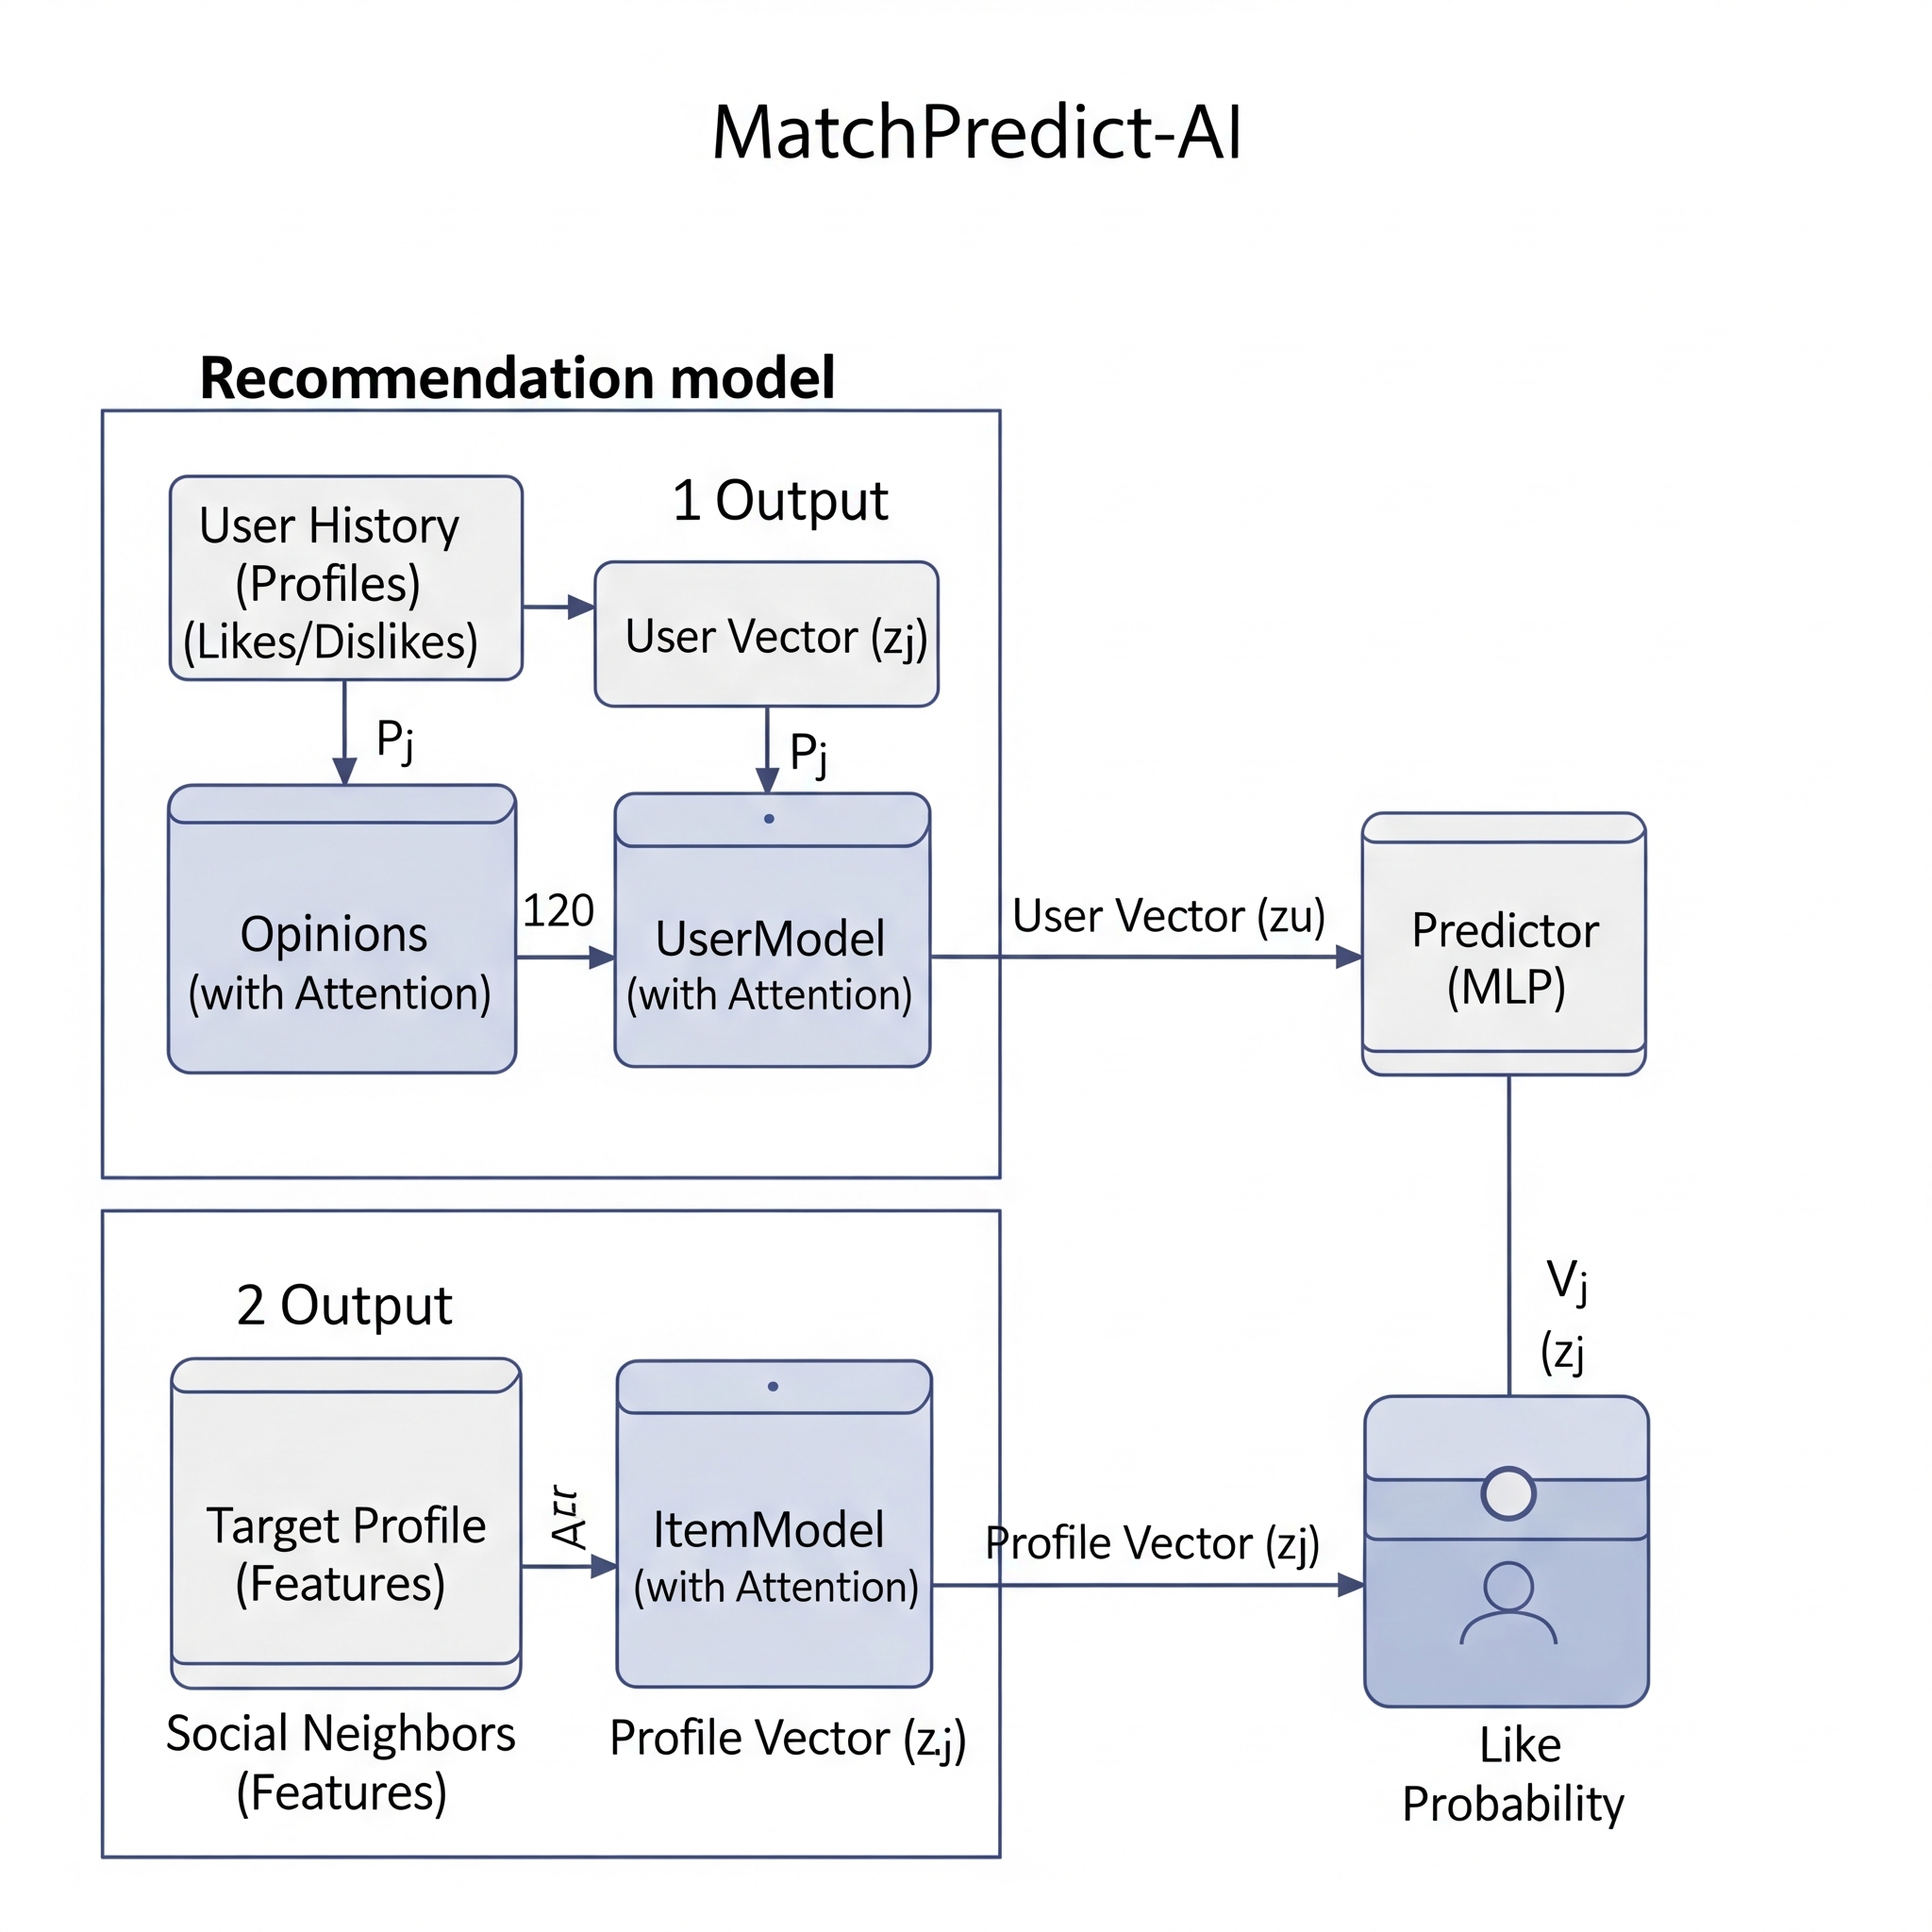
\includegraphics[width=0.8\textwidth]{imagens/diagrama_arquitetura.png} % Lembre-se de criar e adicionar esta imagem
    \caption{Diagrama da arquitetura do modelo MatchPredict-AI, mostrando a interação entre o UserModel (agregando histórico), o ItemModel (agregando vizinhos sociais) e o Predictor final.}
    \label{fig:arquitetura_modelo_tcc2}
\end{figure}

\textbf{Componentes do Modelo:} \\
A arquitetura do GraphRec implementada é modular e pode ser decomposta nos seguintes componentes:

\begin{itemize}
    \item \textbf{ItemModel:}
    \\ \textbf{Objetivo:} Este módulo é responsável por aprender a representação latente final de um perfil-alvo, denotada como $z_j$. A sua função é enriquecer o vetor de features inicial de um perfil, incorporando o contexto de sua "vizinhança social".
    \\ \textbf{Funcionamento:} Ele recebe como entrada o vetor de 2503 dimensões do perfil-alvo e os vetores correspondentes aos seus 10 vizinhos mais próximos no grafo de similaridade. Através de um \textbf{mecanismo de atenção}, o ItemModel aprende a ponderar a importância de cada vizinho. Perfis de vizinhos mais relevantes recebem um peso maior na agregação. As features ponderadas dos vizinhos são então somadas à representação do perfil-alvo. O resultado, $z_j$, é uma representação contextualizada, onde o "significado" de um perfil é influenciado pelos perfis aos quais ele é mais similar.

    \item \textbf{UserModel:}
    \\ \textbf{Objetivo:} Este módulo é projetado para aprender a representação latente do "gosto" de um usuário, denotada como $z_u$. Sua função é capturar as preferências de um usuário a partir de suas interações passadas.
    \\ \textbf{Funcionamento:} A sua entrada é um histórico de perfis com os quais o usuário interagiu (no nosso caso, o histórico simulado pelas personas). O `UserModel` também utiliza um \textbf{mecanismo de atenção} para analisar este histórico. Ele aprende a dar pesos diferentes para cada perfil no histórico, permitindo que o modelo foque nos itens mais representativos do gosto do usuário. As features ponderadas dos itens do histórico são então agregadas para formar o vetor final $z_u$, que sintetiza as preferências daquele usuário.

    \item \textbf{Predictor:}
    \\ \textbf{Objetivo:} Este componente final é responsável por realizar a predição de compatibilidade.
    \\ \textbf{Funcionamento:} Trata-se de uma rede neural do tipo Multi-Layer Perceptron (MLP). Ela recebe como entrada a concatenação dos vetores de usuário ($z_u$) e de item ($z_j$) aprendidos pelos módulos anteriores. Através de suas camadas densas com funções de ativação ReLU, o MLP aprende a relação complexa e não-linear entre o gosto de um usuário e as características de um perfil. A camada de saída do MLP produz um único valor (logit), que é então passado por uma função de ativação sigmoide para gerar a probabilidade final de "like", um valor contínuo entre 0 e 1.
\end{itemize}

\textbf{Justificativa da Escolha:} \\
A escolha da arquitetura GraphRec foi motivada por sua capacidade nativa de lidar com os desafios inerentes a dados de recomendação. Ao contrário de modelos mais simples, ela modela conjuntamente as interações e as relações sociais (ou de similaridade), e os mecanismos de atenção permitem que o modelo aprenda de forma diferencial quais vizinhos e quais itens do histórico são mais importantes, refinando significativamente a qualidade da personalização.
% tex/Desenvolvimento/dev_04_desenho_experimental.tex
\section{Desenho Experimental e Protocolo de Avaliação}
\label{sec:dev_desenho_experimental}

\textbf{Explicação Detalhada:} \\
A avaliação do MatchPredict-AI foi conduzida através de um desenho experimental comparativo, cujo objetivo principal era não apenas medir o desempenho geral do sistema, mas, crucialmente, analisar e quantificar o impacto do contexto do usuário — representado pelo seu histórico de interações — na qualidade das recomendações. Para isolar e investigar este efeito de forma controlada, e devido à ausência de históricos de usuários reais no dataset, foram criadas **personas simuladas**. Esta abordagem permite testar o comportamento do `UserModel` em cenários ideais e de estresse, fornecendo insights valiosos sobre sua robustez e sensibilidade. O protocolo de avaliação foi implementado nos scripts `src/scripts/create_personas.py` e `src/scripts/evaluate_comparison.py`.

\textbf{Justificativa da Abordagem:} \\
A justificativa para esta metodologia baseada em cenários reside na sua capacidade de isolar e medir o efeito do contexto do usuário, uma característica central da proposta de valor do MatchPredict-AI. A comparação direta do desempenho entre os três cenários permite não apenas verificar se o modelo utiliza o histórico, mas também como a qualidade e a natureza desse histórico influenciam a sua eficácia. A validade das conclusões derivadas desta avaliação depende da plausibilidade das personas construídas, que foi validada visualmente no capítulo de resultados (Figura \ref{fig:tsne_personas_tcc2}).

\textbf{Cenários de Teste:}
\begin{itemize}
    \item \textbf{Cenário 1: Baseline (Sem Histórico):}
    \\ \textbf{Descrição:} Neste cenário, o modelo opera sem qualquer informação sobre o histórico de interações do usuário. Para cada predição, o `UserModel` recebe um input neutro (representando uma opinião de 0.5), forçando o sistema a basear sua recomendação unicamente nas features intrínsecas do perfil-alvo e no seu contexto social.
    \\ \textbf{Propósito:} Este cenário serve como um ponto de referência fundamental. Ele estabelece o desempenho do modelo em uma situação de "cold start" (partida a frio), comum para novos usuários em uma plataforma, e permite quantificar o ganho de desempenho que é especificamente atribuível à introdução do contexto do usuário nos cenários subsequentes.

    \item \textbf{Cenário 2: Persona Consistente:}
    \\ \textbf{Descrição:} Este cenário simula um usuário com um histórico de interações coeso e consistente. O `UserModel` é alimentado com um histórico de 20 perfis que são muito similares entre si (selecionados com base na alta similaridade de cosseno com um perfil "âncora").
    \\ \textbf{Propósito:} O objetivo aqui é avaliar a capacidade do `UserModel` de aprender e se adaptar a um padrão de preferência bem definido. Espera-se que, ao processar um histórico consistente, o modelo consiga refinar significativamente suas recomendações para perfis que se alinham com a persona.

    \item \textbf{Cenário 3: Persona Inconsistente:}
    \\ \textbf{Descrição:} Em contraste, a "Persona Inconsistente" simula um usuário cujo histórico de interações é ambíguo e ruidoso. O `UserModel` é alimentado com um histórico de 20 perfis selecionados de forma aleatória e distinta do dataset.
    \\ \textbf{Propósito:} Este cenário visa testar a robustez do modelo frente a dados de entrada sem um padrão discernível. A análise do desempenho busca entender como o `UserModel` lida com sinais contextuais contraditórios, o que é um teste de estresse importante para avaliar a confiabilidade do modelo em situações realistas.
\end{itemize}

\textbf{Métricas de Avaliação:} \\
Para avaliar e comparar o desempenho do MatchPredict-AI nos diferentes cenários, foi utilizado um conjunto padrão de métricas para tarefas de classificação binária:
\begin{itemize}
    \item \textbf{AUC (Area Under the Curve):} Mede a capacidade do modelo de discriminar corretamente entre classes positivas (like) e negativas (dislike), independentemente de um limiar de classificação. É uma excelente medida do poder de ranqueamento do modelo.
    \item \textbf{Acurácia:} Mede a proporção de predições corretas no geral.
    \item \textbf{Precisão:} Avalia, de todas as vezes que o modelo previu "like", quantas estavam corretas. É a métrica da "qualidade" das recomendações positivas.
    \item \textbf{Recall (Sensibilidade):} Mede, de todos os "likes" que realmente existiam, quantos o modelo conseguiu encontrar. É a métrica da "abrangência" das recomendações.
    \item \textbf{F1-Score:} A média harmônica entre Precisão e Recall, fornecendo uma métrica única que equilibra ambas.
\end{itemize}